% Chapter Template

\chapter{La piattaforma ARM embedded} % Main chapter title

\label{Chapter5} % Change X to a consecutive number; for referencing this chapter elsewhere, use \ref{ChapterX}

\lhead{Capitolo 5. \emph{La piattaforma ARM embedded}} % Change X to a consecutive number; this is for the header on each page - perhaps a shortened title

%----------------------------------------------------------------------------------------
%	SECTION 1
%----------------------------------------------------------------------------------------

\section{Sistema \emph{embedded}}

%Sistema embedded: che cos'è, a che cosa serve, chi rientra nella categoria?
%Differenza tra special purpose e general purpose, importanza dell'applicazione
// Rivedere questo incipit \\
Un sistema può essere visto come un insieme di più parti che collaborano al fine
di svolgere un determinato compito; considerando gli  ambiti informatici ed 
elettronici un sistema \emph{embedded} (tradotto solitamente con ``sistema 
integrato'') 

%----------------------------------------------------------------------------------------
%	SECTION 2
%----------------------------------------------------------------------------------------

\section{Processori ARM}

%-----------------------------------
%       SUBSECTION 1
%-----------------------------------

\subsection{Il processore AllWinner A20}

%----------------------------------------------------------------------------------------
%       SECTION 3
%----------------------------------------------------------------------------------------

\section{Il \emph{single-board} computer Banana Pi M1}
\begin{center}
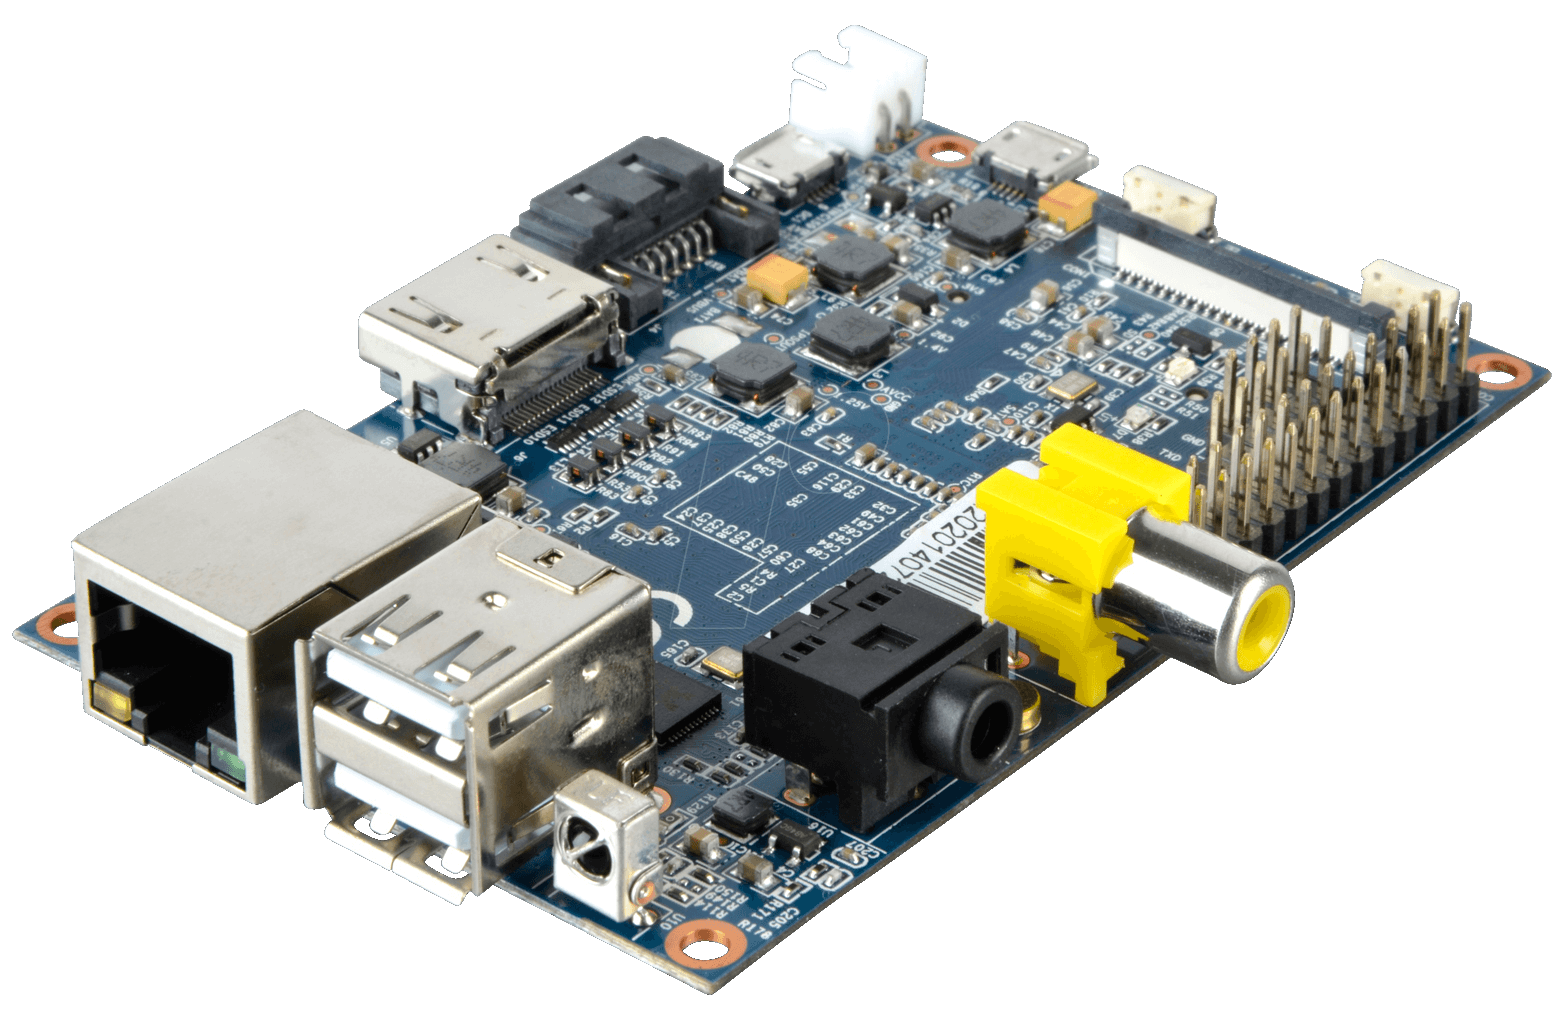
\includegraphics[scale=0.175]{Figures/bananapi.png}\\[0.5cm]
\end{center}